\nonumchapter{总复习题}

\begin{xiaotis}

\xiaoti{填空:\\
    \begin{tblr}{hlines, vlines, columns={c}, column{1-6,8}={2em}}
        符号 & \ce{O2} & \ce{2O} & \ce{S^{2-}} & $\overset{-2}{\ce{S}}$ & \ce{HgO}
            & \ce{2CO2} & \Charge{0=\., 90=\:, 180=\:, 270=\:}{Cl}
            & \chemfig{
                Na^+
                \chemleft[\setcharge{extra sep=3pt}\Charge{0=\:, 90=\:, 180=\chargexdot, 270=\:}{Cl}\chemright]^{-}
            } \\
        表示 &
    \end{tblr}
}


\xiaoti{选择正确的答案填写在括号里。}
\begin{xiaoxiaotis}

    \xxt{在 \ce{H2O} 和 \ce{H2SO4} 各 5 个分子里含 \ewkh 一样多。\\
        \tc{1} 氢分子, \tc{2} 氢原子, \tc{3} 氢元素, \tc{4} 氢元素的百分率。
    }

    \xxt{纯碱 \ewkh, 熟石灰 \ewkh, 硫酐 \ewkh, 氧化铁 \ewkh.氧化铝 \ewkh, 汞 \ewkh。\\
        \tc{1} 碱, \tc{2} 酸, \tc{3} 酸性氧化物, \tc{4} 正盐, \tc{5} 酸式盐, \tc{6} 两性氧化物,
        \tc{7} 碱性氧化物, \tc{8} 单质, \tc{9} 碱式盐。
    }

    \xxt{\ewkh 是电解质。\\
        \tc{1} 酒精, \tc{2} 固体氯化钠, \tc{3} 铜丝。
    }

\end{xiaoxiaotis}


\xiaoti{下列的说法有没有错误? 说明理由。}
\begin{xiaoxiaotis}

    \xxt{原子是最小的微粒。}

    \xxt{空气是由几种单质组成的混和物。}

    \xxt{一个氧原子的质量就是氧的原子量。}

    \xxt{饱和溶液析出晶体后就变成不饱和溶液。}

    \xxt{能跟酸起反应的氧化物就是碱性氧化物。}

    \xxt{根据质量守恒定律,参加化学反应的各物质的质量总和,等于反应后生成的各物质的质量总和,所以 8 克氧气跟 5 克碳起反应能生成 13 克二氧化碳。}

\end{xiaoxiaotis}


\xiaoti{回答下列问题。}
\begin{xiaoxiaotis}

    \xxt{画出下列符号所代表的原子或离子结构的示意图(符号左下角的数字为核电荷数)。\\
        \tc{1} $_{11}A$, \tc{2} $_{16}B$, \tc{3} $_{17}C^-$, \tc{4} $_{18}D$, \tc{5} $_{19}E^+$。
    }

    \xxt{写出上列各示意图所代表的微粒的名称。}

    \xxt{用电子式表示 $A$ 和 $B$ 两种微粒形成分子的过程。}

    \xxt{由 $C^-$ 和 $E^+$ 两种微粒所组成的化合物是共价化合物吗? 它的水溶液能不能导电?}

    \xxt{举出由 $D$ 元素所组成的单质的一种用途。}

\end{xiaoxiaotis}


\xiaoti{下列各式有没有错误? 说明理由。}
\begin{xiaoxiaotis}

    \xxt{\ce{ CaCO3 + Cu(OH)2 = CuCO3 + Ca(OH)2 }}

    \xxt{\ce{ H2O = H2 + O }}

    \xxt{\ce{ Cu + H2SO4 = CuSO4 + H2 ^ }}

    \xxt{\ce{ CuO + H2O = Cu(OH)2 }}

    \xxt{\ce{ Fe + ZnCl2 = FeCl3 + Zn }}

    \xxt{\ce{ CO + Fe2O3 = Fe + CO2 }}

    \xxt{\ce{ NaOH + KNO3 = KOH + NaNO3 }}

    \xxt{\schemestart
        \setcharge{extra sep=3pt}
        \chemfig{\charge{0=\chargex}{H}}
        \+
        \chemfig{\charge{0=\:, 90=\:, 180=\., 270=\:}{Cl}}
        \; =
        \chemfig{
            H^+
            \chemleft[\setcharge{extra sep=3pt}\Charge{0=\:, 90=\:, 180=\chargexdot, 270=\:}{Cl}\chemright]^{-}
        }
    \schemestop}

\end{xiaoxiaotis}


\xiaoti{用化学方程式表示下列各反应,并注明反应类型。如果属于复分解反应,要说明反应可以发生的原因;
    如果属于氧化-还原反应,要指出氧化剂和还原剂。
}
\begin{xiaoxiaotis}

    \begin{tblr}{}
        \xxt{加热高锰酸钾,}   &  \xxt{纯碱跟盐酸,} \\
        \xxt{生石灰跟水,}    &  \xxt{氢氧化钾跟盐酸,} \\
        \xxt{硝酸银跟氯化钠,}  & \xxt{二氧化碳通入石灰水,} \\
        \xxt{铁片跟稀盐酸,} & \xxt{点燃爆鸣气,} \\
        \xxt{氯化钡跟硫酸钠,} &  \xxt{锌跟氯化铁。}
    \end{tblr}

\end{xiaoxiaotis}


\xiaoti{按下列各题的要求分别写出一个氧化-还原反应的化学方程式,说明反应前后元素化合价的变化情况。}
\begin{xiaoxiaotis}

    \xxt{一种单质 $+$ 另一种单质(其中一种单质是氧化剂)}

    \xxt{单质 $+$ 化合物(单质是氧化剂)}

    \xxt{单质 $+$ 化合物(单质是还原剂)}

\end{xiaoxiaotis}


\xiaoti{试用锌粒、氧化铜和稀硫酸作原料,用两种不同的方法制取铜。写出有关反应的化学方程式。}

\xiaoti{在铁、稀硫酸、氧化铝、氯化铜溶液和氢氧化钠溶液中,在常温下,哪两种物质间能发生化学反应?写出有关反应的化学方程式。}

\xiaoti{现有氢气、氧气、空气、氮气和二氧化碳等五种无色气体各一瓶,试用实验方法把它们一一鉴别出来。}

\xiaoti{有人用一种无色溶液进行了下列两个实验:\\
    (a) 取该溶液少许, 在溶液里滴入几滴酚酞试液,溶液无变化。 \\
    (b) 取两支试管,各倒入该溶液少许。在其中一支试管里投入两小粒锌,发现有无色无味的气体放出。该气体能燃烧,火焰呈淡蓝色。
        在另一支试管里滴加氯化钡溶液,发现有白色沉淀生成,再加入稀硝酸,沉淀不溶解。 \\
    根据上述实验现象你认为这是什么溶液?写出溶质的分子式,并写出有关反应的化学方程式。
}


\xiaoti{有一包白色固体,可能是氯化钙和碳酸钠的混和物,也可能只含其中一种物质。为了鉴别它,做了下列实验:\\
    (a) 取一些白色固体溶在水里,有白色沉淀生成。把该悬浊液过滤,滤液无色。 \\
    (b) 在滤出的沉淀里加入盐酸,有无色气体生成。该气体能使澄清的石灰水变浑浊。 \\
    (c) 在滤液里加入硝酸银溶液,有白色沉淀生成,再加入稀硝酸,沉淀不溶解。\\
    根据上述实验现象判断:
}
\begin{xiaoxiaotis}

    \xxt{这白色固体是什么物质,}

    \xxt{操作 (a) 里滤出的白色沉淀是什么物质?}

    \xxt{滤液里含有哪些溶质的离子?}

    \hspace*{2em} 写出有关反应的化学方程式。

\end{xiaoxiaotis}


\xiaoti{把氯化氢、氢氧化钠、氯化钠、三氧化硫和氧化钙分别溶于水,在它们的水溶液里分别滴入几滴紫色石蕊试液。填空:}
\begin{xiaoxiaotis}

    \xxt{$\text{pH 值} > 7$ 的溶液是 \xhx[5em] , 石蕊试液显 \xhx 色。}

    \xxt{$\text{pH 值} < 7$ 的溶液是 \xhx[5em] , 石蕊试液显 \xhx 色。}

    \xxt{$\text{pH 值} = 7$ 的溶液是 \xhx[5em] , 石蕊试液显 \xhx 色。}

\end{xiaoxiaotis}


\xiaoti{解释下列问题:}
\begin{xiaoxiaotis}

    \xxt{炉火用扇子扇, 越扇越旺, 蜡烛火焰却一扇就灭,为什么?}

    \xxt{用墨写的字或作的画能保存多年不褪色,为什么?}

    \xxt{熟石灰经过长期存放会变质,为什么?}

    \xxt{做馒头时,面团经过发酵会生成一些酸,这时可以加一些纯碱溶液,用力揉和,然后做成馒头,加热蒸熟。蒸熟的馒头为什么会变得疏松多孔?}

    \xxt{施用碳酸氢铵肥料时必须用土把它覆盖,为什么?}

    \xxt{施用氨水肥料时必须先把它稀释,为什么?}

\end{xiaoxiaotis}


\xiaoti{下列操作有没有错误? 为什么? 如有错误, 应怎样改正?}
\begin{xiaoxiaotis}

    \xxt{试管口对着人加热。}

    \xxt{给盛有液体体积超过三分之一的试管加热。}

    \xxt{不垫石棉网, 把烧杯放在铁环上直接加热。}

    \xxt{用燃着的酒精灯去点燃另一个酒精灯。}

    \xxt{用手直接拿砝码。}

    \xxt{把药品直接放在天平的托盘上称量。}

    \xxt{用漏斗过滤时液面高于滤纸的边缘。}

    \xxt{把水迅速地倒在盛浓硫酸的量筒里。}

\end{xiaoxiaotis}


\xiaoti{现有氯酸钾、二氧化锰、锌粒、盐酸和大理石五种物质。}
\begin{xiaoxiaotis}

    \xxt{怎样利用这些物质用实验室方法制取常见的三种气体? 写出有关反应的化学方程式。}

    \xxt{画出制取这三种气体所选用的发生装置和收集装置。说明选用它们的理由。}

\end{xiaoxiaotis}


\xiaoti{填空:}
\begin{xiaoxiaotis}

    \xxt{1 吨尿素 〔 \ce{CO(NH2)2} 〕里含氮 \xhx[3em] 吨。}

    \xxt{煅烧 10 吨碳酸钙可制得 \xhx[3em] 吨生石灰和 \xhx[3em] 吨二氧化碳。}

    \xxt{20 ℃ 时硝酸钾的溶解度是 $31.6$ 克, 50 克 20 ℃ 的硝酸钾饱和溶液里含有 \xhx[3em] 克硝酸钾,
        它的百分比浓度是 \xhx[3em] 。如果把这溶液稀释到 $10\%$, 需加水 \xhx[3em] 毫升。
    }

\end{xiaoxiaotis}


\xiaoti{通过计算说明:}
\begin{xiaoxiaotis}

    \xxt{在两个烧杯里各倒入 20 克 $20\%$ 的硫酸溶液,然后分别加入 5 克锌片和 5 克铁片。
        等反应完毕后,烧杯里剩余物质的质量是否相等?
    }

    \xxt{如果最初在烧杯里各倒入 50 克 $20\%$ 的硫酸溶液,而加入的锌片和铁片的质量不变,
        等反应完毕后,烧杯里剩余物的质量是否相等?
    }

    \hspace*{2em}(假设在上述两种情况下生成的气体全部从溶液中逸出。)

\end{xiaoxiaotis}


\xiaoti{有人利用氢气还原灼热氧化铜的实验来测定水的组成(实验装置见图), 得到下列结果:\\
    氧化铜和玻璃管在通入氢气前的总质量是 $65.6$ 克;\\
    氧化铜和玻璃管在通入氢气完反应后的总质量是 $59.2$ 克;\\
    氯化钙和 U 型管在实验前的总质量是 $100.8$ 克;\\
    氯化钙和 U 型管在实验后的总质量是 $108.0$ 克。求:
}
\begin{figure}[H]
    \centering
    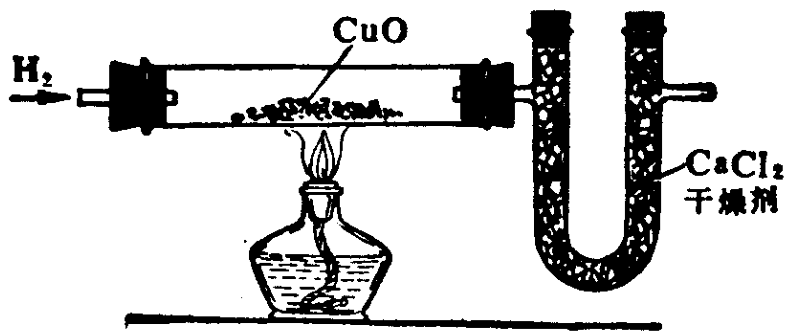
\includegraphics[width=8cm]{../pic/czhx1-zfx-19.png}
\end{figure}

\begin{xiaoxiaotis}

    \xxt{完全反应后生成水的质量。}

    \xxt{在生成的水中的氧的质量。}

    \xxt{在生成的水中的氢的质量。}

    \xxt{水中氢跟氧的质量比。}

\end{xiaoxiaotis}


\xiaoti{把 $6.1$ 克干燥纯净的氯酸钾和二氧化锰的混和物放在试管里加热,直到氯酸钾完全分解为止。
    冷却后,称得剩余固体物质的质量为 $4.2$ 克。问:
}
\begin{xiaoxiaotis}

    \xxt{反应后制得氧气多少克? 这些氧气在标准状况下的体积是多少?}

    \xxt{剩余的固体物质是什么? 它们的质量分别是多少克?}

    \xxt{原混和物里含氯酸钾多少克?}

\end{xiaoxiaotis}


\xiaoti{实验室里用一氧化碳还原赤铁矿(主要成分是 \ce{Fe2O3})样品 3 克,
    反应生成的二氧化碳跟过量的石灰水起反应生成的白色沉淀重 4 克。
    求赤铁矿里含 \ce{Fe2O3} 的百分率。
}


\xiaoti{氯化钠和硝酸钾在不同温度下的溶解度如下:\\
    \begin{tblr}{hlines, vlines, columns={c}}
        \diagboxthree{物质}{溶解度}{温度} & 0 ℃ & 10 ℃ & 20 ℃ & 30 ℃ & 40 ℃ & 60 ℃ & 80 ℃ & 100 ℃ \\
        \ce{NaCl} &  35.7 & 35.8 & 36.0 & 36.3 & 36.6 & 37.3 & 38.4 & 39.8 \\
        \ce{KNO3} &  13.3 & 20.9 & 31.6 & 45.8 & 63.9 & 110  & 169  & 246
    \end{tblr}
}
\begin{xiaoxiaotis}

    \xxt{用什么方法可以把硝酸钾从它和氯化钠的混和物里分离出来,}

    \xxt{如果需要从 40 ℃ 的氯化钠饱和溶液 300 克中获得 50 克氯化钠晶体, 应蒸发掉多少克水?}

    \xxt{如果需要从 100 ℃ 的硝酸钾饱和溶液 522 克中获得 302 克硝酸钾晶体,应把溶液冷却到什么温度?}

    \xxt{上述溶液析出 302 克硝酸钾晶体后,该溶液的百分比浓度是多少?}

\end{xiaoxiaotis}


\xiaoti{把一块重 82 克的极薄的纯净铁片浸入 342 克硫酸铜溶液,等反应完毕后(假定这时硫酸铜里的铜已全部析出),
    把附有铜的铁片从溶液中取出。洗净,干燥,再称量,得 $83.5$ 克。问:
}
\begin{xiaoxiaotis}

    \xxt{铁片上附有多少克铜?}

    \xxt{原硫酸铜溶液的百分比浓度是多少?}

\end{xiaoxiaotis}

\end{xiaotis}

